\documentclass[11pt,a4paper]{report}
\usepackage[utf8]{inputenc}
\usepackage[french]{babel}
\usepackage[T1]{fontenc}
\usepackage{amsmath}
\usepackage{amsfonts}
\usepackage{amssymb}
\usepackage{xcolor}
\usepackage{gensymb}

\usepackage{geometry}
\geometry{hmargin=2.5cm,vmargin=1.5cm}
\usepackage{wasysym}
\usepackage{graphicx}

\author{Mathieu Sarrat}
\title{LC11 - Solvants}

\makeatletter
\renewcommand{\thesection}{\@arabic\c@section}
\makeatother


\begin{document}
\maketitle

\section*{Niveau, Pré-requis et objectifs}
\begin{itemize}
	\item \textbf{Niveau :} PTSI\\
	
	\item \textbf{Pré-requis :}
	\begin{itemize}
		\item Classification périodique;
		\item Représentation de Lewis, liaison covalente;
		\item Liaison polarisée, molécule polaire et moment dipolaire.\\
	\end{itemize}
	
	\item \textbf{Objectifs :}
	\begin{itemize}
		\item Lier qualitativement la valeur plus ou moins grande des forces intermoléculaires à la 			polarité et la polarisabilité des molécules;
		\item Prévoir ou interpréter les propriétés physiques de corps purs par l'existence 					d'interactions de van der Waals ou de liaisons hydrogène intermoléculaires; 
		\item Interpréter la miscibilité ou la non-miscibilité de deux solvants;
		\item Justifier ou proposer le choix d'un solvant adapté à la dissolution d'une espèce 					donnée, à la réalisation d'une extraction et aux principes de la chimie verte.\\
	\end{itemize}
		
	\item \textbf{Recommandations :}
	\begin{itemize}
		\item Pas plus de 10 minutes sur la première partie (diapos, messages forts). Passer les 					interactions de van der Waals en rappel;
		\item Faire des schémas pour déterminer graphiquement le moment dipolaire d'un solvant comme 				l'eau ou l'acétone (montrer par flexcam, ou faire une diapo s'il reste du temps);
		\item Pour l'extraction de l'acide propanoïque : que le dosage en direct. On fait déjà les 					gestes expérimentaux avec le diiode.
	\end{itemize}
\end{itemize}

\newpage
\section*{Introduction}

En chimie, les solvants sont utilisés pour dissoudre, diluer extraire d'autres substances sans les modifier chimiquement. Les solvants sont utilisés dans des secteurs très diversifiés tels que les peintures, les encres, le nettoyage (détergents) ou encore la synthèse organique. Le rôle d'un solvant est de permettre la rencontre des molécules réagissant dans une réaction : une réaction est très influencée par la nature du solvant dans laquelle elle se déroule. Le choix d'un solvant ne se fait donc pas au hasard, car toutes les molécules ne sont pas solvatées de la même façon par tous les solvants.\\

On peut expliquer microscopiquement les propriétés d'un solvant à travers les interactions que les molécules le constituant établissent avec les molécules des solutés. Ces interactions sont faibles et ne sont donc pas les liaisons covalentes et les liaisons ioniques que nous avons introduites lors du cours précédent. Elles sont néanmoins très importantes pour expliquer certaines propriétés de la matière. Deux exemples :
\begin{itemize}
	\item elles sont responsables de la structure hélicoïdale de la molécule d'ADN,
	\item elles sont responsables de la non-miscibilité de certains liquides entre eux, comme l'eau 			et l'huile,
	\item elles sont à l'origine des effets de tension superficielle que l'on peut remarquer dans la 		vie de tous les jours, par exemple la forme des gouttes d'eau.\\ 
\end{itemize}

Nous allons répertorier et décrire ces interactions dans un premier temps, ainsi que certaines de leurs conséquences visibles. Nous utiliserons ensuite ces connaissances pour comprendre le rôle d'un solvant (constituant très largement majoritaire) dans une solution et définir un certain nombre de propriétés pour les solvants.

\newpage
\section{Les interactions faibles}\label{sec:1}

\subsection{Nécessité expérimentale}

Au sein des molécules, nous avons vu que ce sont des liaisons fortes, comme la liaison covalente ou la liaison ionique qui assurent la cohésion entre les atomes. L'ordre de grandeur des énergies en jeu est quelques centaines de kJ/mol.\\

Contrairement aux gaz dilués, \textbf{les molécules en phase liquide ou dans les solides moléculaires} (comme la glace d'eau ou encore la glace carbonique) \textbf{ne sont pas libres :} elles interagissent entre elles, ce qui assure la cohésion de la matière : on parle de forces intermoléculaires. Lorsqu'on regarde les énergies associées aux \textbf{chaleurs latentes} de fusion et de vaporisation, on remarque qu'elles sont \textbf{bien inférieures aux énergies des liaisons covalentes}. Les forces intermoléculaires sont donc qualifiées de liaisons faibles, ou d'interactions faibles.

\begin{figure}[h!]
	\begin{center}
	\begin{tabular}{cc}
			
	\begin{tabular}{|c|c|}
		\hline
		Liaison & Énergie (kJ/mol)\\
		\hline
		O-H & 464\\
		\hline
		C-H & 414\\
		\hline
		C-C & 347\\
		\hline
		C$=$C & 615\\
		\hline 
		C-O & 351\\
		\hline
		C=O & 730\\
		\hline
		C-Cl & 331\\
		\hline
		C-N & 293\\
		\hline
		C$=$N & 615\\
		\hline
		C$\equiv$N & 890\\
		\hline
		Br-Br & 192\\
		\hline 
	\end{tabular}
			
	&
	
	\begin{tabular}{|c|c|c|}
		\hline
		Liaison & Fusion (kJ/mol) & Ébullition (kJ/mol)\\
		\hline
		$\text{H}_2$ & 0.12 & 0.94\\
		\hline
		$\text{O}_2$ & 1.84 & 1.63\\
		\hline
		$\text{N}_2$ & 0.71 & 5.44\\
		\hline
		$\text{H}_2\text{O}$ & 6.01 & 40.7\\
		\hline
		$\text{CO}_2$ & 8.63 & 25.13\\
		\hline
		Éthanol & 4.60 & 38.91\\
		\hline 
		Acide acétique & 11.72 & 24.27\\
		\hline
		$\text{NH}_3$ & 5.65 & 23.35\\
		\hline
		$\text{F}_2$ & 1.55 & 6.27\\
		\hline
		$\text{Cl}_2$ & 6.28 & 20.42\\
		\hline
		$\text{Br}_2$ & 10.88 & 30.96\\
		\hline
		$\text{I}_2$ & 15.48 & 43.51\\
		\hline 
	\end{tabular}
	\end{tabular}
	\end{center}
	\caption{Énergies de liaison (gauche) et chaleurs latentes (droite) : ordres de grandeur.}
\end{figure}

Regardons de plus près une même famille de composés chimiques : les dihalogènes. A température et pression ambiantes, le difluor et le dichlore sont des gaz, le dibrome est liquide et le diiode est solide. Si on regarde les chaleurs latente de fusion et de vaporisation de ces composés, on remarque qu'elles augmentent avec la taille des molécules.\\

\begin{figure}[h!]
	\begin{center}
		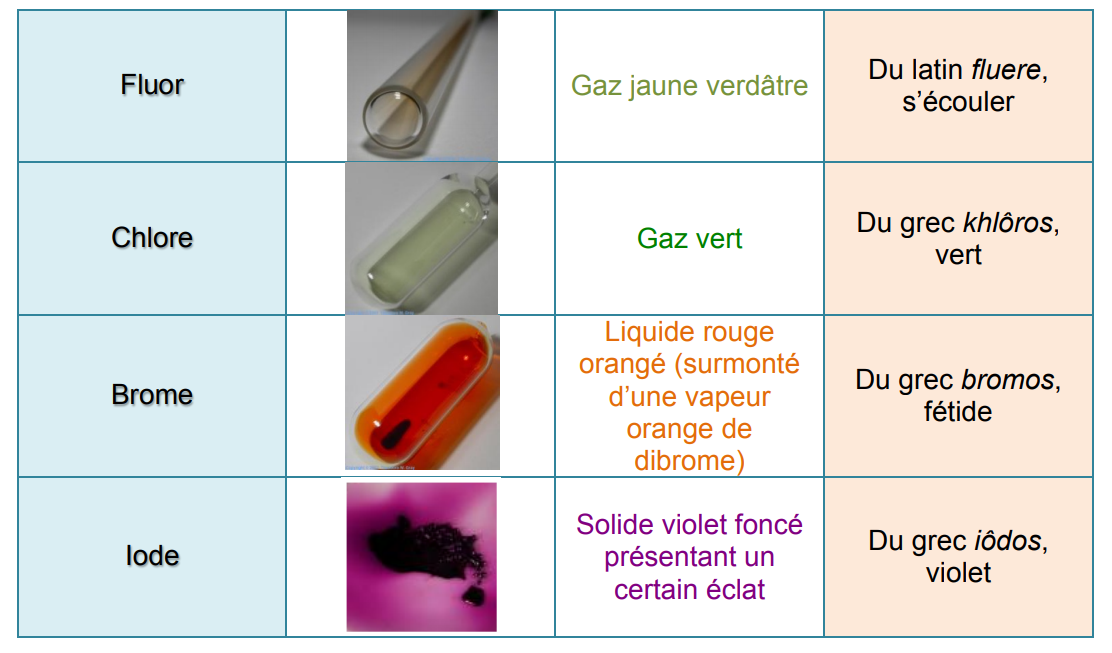
\includegraphics[scale = 0.45]{dihalos.png}
	\end{center}
	\caption{Les dihalogènes sous les conditions standard de température et de pression.}
\end{figure}

\subsection{Les liaisons de van der Waals}

Nous avons vu que certaines molécules, comme l'eau, possédaient un moment dipolaire : le barycentre des charges positive et celui des charges négative ne coïncident pas, du fait des différences d'électronégativé entre les atomes constituant la molécule. Ces \textbf{molécules se comportent comme des dipôles électrostatiques}. En conséquence :
\begin{itemize}
	\item elles produisent un champ électrique dans leur voisinage,
	\item elles sont capables d'interagir avec un champ électrique extérieur, par exemple celui 				généré par une autre molécule dipolaire.
\end{itemize}

Les molécules vont donc pouvoir interagir entre elles du fait de leur moment dipolaire. On associe une énergie à ces interactions, et on admettra qu'elle est une fonction de la distance séparant les deux dipôles. On dénombre \textbf{trois types d'interaction dipolaire attractives}.

\subsubsection{Interaction de Keesom}

\textbf{Deux dipôles permanents} peuvent interagir entre eux à travers l'interaction de Keesom. On retrouvera donc cette interaction en présence de deux molécules d'eau, ces molécules ayant un moment dipolaire permanent du fait de leur géométrie. L'énergie potentielle associée à l'interaction de Keesom a la forme suivante
\begin{equation}
	E_K = - \frac{C_K}{r^6}.
\end{equation}
Elle décroît donc très vite par rapport à l'interaction coulombienne entre deux charges ponctuelles (qui est en $1/r^2$). \textbf{Le signe moins implique une interaction attractive}.

\subsubsection{Interaction de Debye}

Un dipôle permanent lorsqu'il s'approche d'une molécule apolaire (pas de moment dipolaire permanent) est capable d'induire un dipôle grâce au champ électrique qu'elle émet. Le moment dipolaire créé est proportionnel au champ électrique
\begin{equation}
	\bold{\mu} = \alpha \bold{E},
\end{equation}
avec $\alpha$ la \textbf{polarisabilité} de la molécule. Le dipôle induit sera d'autant plus important que la molécule est facile à polariser ($\alpha$ importante). La \textbf{polarisabilité} d'une molécule dépend notamment de sa taille : les électrons des couches externes d'atomes volumineux sont moins fortement liés au noyau que ceux de plus petits atomes, et donc plus faciles à déplacer. La molécule de diiode aura une polarisabilité plus importante que celle de dibrome, elle même plus polarisable que le dichlore.\\

On appelle interaction de Debye, l'interaction entre un dipôle permanent et un dipôle induit. L'énergie potentielle associée à cette interaction \textbf{attractive} s'écrit
\begin{equation}
	E_D = -\frac{C_D}{r^6}.
\end{equation} 

\subsubsection{Interaction de London}

Il est possible de liquéfier des gaz constitués de molécules apolaires, comme $\text{H}_2$ ou $\text{He}$ ou encore $\text{N}_2$. Nous avons également vu que le diiode était un solide et le dibrome un liquide à température ambiante. Il est donc possible d'observer des phases condensées constituées de molécules apolaires, donc incapables d'établir des interactions de type Keesom ou Debye.\\

Du fait de la faible masse des électrons vis à vis des noyaux, les électrons sont toujours en mouvement : à chaque instant, toute molécule apolaire présente un moment dipolaire instantané, bien que la moyenne temporelle de ce moment soit nulle. La \textbf{moyenne des interactions entre dipôles instantanés} d'une molécule avec ses voisines est appelée  \textbf{interaction de London} ou encore \textbf{interaction de dispersion} :
\begin{equation}
	E_L = -\frac{C_L}{r^6}.
\end{equation}
Cette interaction est attractive et \textbf{augmente avec la polarisabilité des molécules}.

\subsubsection{Énergie totale d'interaction}

On somme les contributions des trois interactions que nous venons de décrire :
\begin{equation}
	E_\text{VdW} = -\frac{C_K + C_D + C_L}{r^6} = -\frac{C}{r^6}.
\end{equation}

\textbf{Pour la plupart des corps purs}, ce sont les \textbf{interactions de London qui dominent}. L'eau est une exception : petite molécule possédant un très fort moment dipolaire permanent, ce sont les interactions de Keesom qui prédominent dans son cas. Les interactions de Keesom ne sont pas non plus négligeables dans le cas de l'ammoniac \textcolor{red}{(CF. Tableau en Figure 3)}. Le poids des interactions de London est plus élevé pour HI que pour HCl, la molécule étant plus polarisable du fait de la présence de l'atome d'iode, plus volumineux que celui de chlore.\\

\'A cette énergie potentielle attractive s'ajoute une dernière contribution, cette fois-ci de nature répulsive : à très courte distance, les molécules se repoussent, du fait de l'impénétrabilité des nuages électroniques. On retient souvent un potentiel répulsif de la forme
\begin{equation}
	E_\text{Rep} = \frac{A}{r^{12}}
\end{equation}
pour modéliser cet effet, d'où l'expression et la forme de l'\textbf{énergie potentielle totale d'interaction entre deux molécules :}
\begin{equation}
	\boxed{E_p = E_\text{VdW} + E_\text{Rep} = \frac{A}{r^{12}} -\frac{C}{r^6}}.
\end{equation}

\begin{figure}[h!]
	\begin{center}
	\begin{tabular}{cc}
	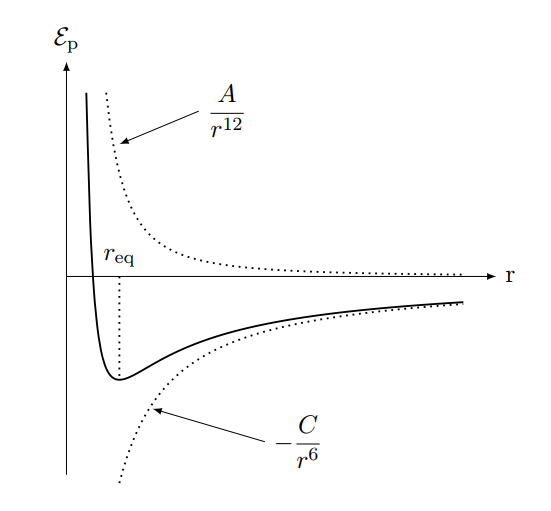
\includegraphics[scale = 0.4]{vanderwaals.png}	
	&
	\begin{tabular}{|c|c|c|c|}
	\hline	
	Corps pur & \% Keesom & \% Debye & \% London \\
	\hline
	Ne & 0 & 0 & 100 \\
	\hline
	HCl & 9 & 5 & 86\\
	\hline
	HI & 0.1 & 0.5 & 99.4\\
	\hline
	$\text{NH}_3$ & 34 & 9 & 57\\
	\hline
	$\text{H}_2\text{O}$ & 69 & 7 & 24\\
	\hline
	\end{tabular}
	\end{tabular}
	\end{center}
	\caption{Gauche : forme de l'énergie potentielle associée aux liaisons faibles. Droite : 				contributions relatives des interactions de Van der Waals pour plusieurs corps purs}
\end{figure}


Le \textbf{minimum} de cette fonction correspond à la \textbf{position d'équilibre} et donne la longueur typique d'une liaison faible. La profondeur maximale du puits de potentiel donne un ordre de grandeur de l'énergie qu'il faut fournir pour briser ces liaisons : \textbf{de 1 à 10 kJ/mol}. La distance typique séparant deux molécules reliées par une liaison faible et de 300 à 500pm.

\subsubsection{Conséquences des liaisons de Van der Waals}

\begin{itemize}
\item \textbf{Chaleurs latentes} et \textbf{températures de fusion et de vaporisation des corps purs} : plus les molécules d'un corps pur sont volumineuses, plus elles sont polarisables, plus les interactions de van der Waals sont fortes, plus la cohésion des molécules en phase condensée est importante. Ceci implique des chaleurs latentes de fusion et d'ébullition de plus en plus élevées ainsi que des températures de fusion et d'ébullition plus importantes.\\
	
\begin{figure}[h!]
	\begin{center}
	\begin{tabular}{cc}
	\begin{tabular}{|c|c|c|}
		\hline
		Composé & $T_{fus} (K)$ & $T_{éb} (K)$ \\
		\hline
		He & 3 & 4\\
		\hline
		Ne & 24 & 27\\
		\hline
		Ar & 84 & 87\\
		\hline
		Kr & 117 & 120\\
		\hline 
		Xe & 161 & 165\\
		\hline
	\end{tabular}	
	&
	\begin{tabular}{|c|c|c|c|c|}
		\hline
		Corps pur & $\text{CH}_4$ & $\text{SiH}_4$ & $\text{GeH}_4$ & $\text{SnH}_4$\\
		\hline
		$T_\text{éb} (\degree C)$ & -161.6 & -111.4 & -88.5 & -52.0 \\
		\hline
		\hline
		\hline
		Corps pur & $\text{NH}_3$ & $\text{PH}_3$ & $\text{AsH}_3$ & $\text{SbH}_3$\\
		\hline
		$T_\text{éb} (\degree C)$ & \textcolor{red}{-33.5} & -87.8 & -62.5 & -17.0\\
		\hline
		\hline
		\hline
		Corps pur & $\text{H}_2\text{O}$ & $\text{H}_2\text{S}$ 
			& $\text{H}_2\text{Se}$ & $\text{H}_2\text{Te}$\\
		\hline
		$T_\text{éb} (\degree C)$ & \textcolor{red}{100.0} & -60.2 & -41.4 & -2.2\\
		\hline
		\hline
		\hline
		Corps pur & $\text{HF}$ & $\text{HCl}$ & $\text{HBr}$ & $\text{HI}$\\
		\hline 
		$T_\text{éb} (\degree C)$ & \textcolor{red}{19.5} & -85.1 & -66.8 & -35.4\\
		\hline
	\end{tabular}
	\\
	\begin{tabular}{|c|c|}
		\hline
		Composé & $T_\text{éb} (K)$ \\
		\hline
		$\text{CH}_4$ & 111.7 \\
		\hline
		$\text{C}_2\text{H}_6$ & 184.6 \\
		\hline
		$\text{C}_3\text{H}_8$ & 231.1 \\
		\hline
	\end{tabular}
	& 
	\end{tabular}
	\end{center}
	\caption{Températures de changement d'état de plusieurs corps purs, classés par familles : en 			haut à gauche, gaz nobles ; en haut à droite colonne du carbone, de l'azote, de l'oxygène et du 		fluor ; en bas à gauche, alcanes.}
\end{figure}	
	
	
	
	
\item Les gaz rares \textcolor{red}{(cf. tableau)} et les dihalogènes vérifient particulièrement 	bien ce comportement : on comprend ainsi pourquoi $\text{I}_2$ est solide, pourquoi $\text{Br}_2$ est liquide et pourquoi	$\text{Cl}_2$ et le $\text{F}_2$ sont gazeux à température ambiante.\\

\item De même, la température d'ébullition des alcanes augmente avec la taille des molécules. \textcolor{red}{(cf. tableau)}.\\	
\end{itemize}

\subsection{La liaison hydrogène}

\subsubsection{Nécessité, définition, caractéristiques}
\begin{itemize}
	\item Par rapport au tableau précédent : on remarque des \textbf{anomalies avec l'eau, 					l'ammoniac et le fluorure d'hydrogène}, toutes trois caractérisées par des températures 				d'ébullition bien supérieures aux espèces de géométrie similaire. Cette anomalie n'est pas 				constatée avec le carbone. On s'attend à ce que les \textbf{atomes d'oxygène, d'azote et de 			fluor, très électronégatifs}, soient capables de participer à \textbf{un autre type de liaison 			faible}.\\
	
	\item \textcolor{blue}{Définition :} on appelle \textbf{liaison hydrogène} l'interaction 				\textbf{attractive} qui se développe \textbf{entre l'hydrogène d'une espèce A-H et le doublet 			non liant d'un atome B. A et B doivent être des atomes fortement électronégatifs (oxygène, azote 	ou fluor)}.\\
	
	\begin{figure}[h!]
	\begin{center}
		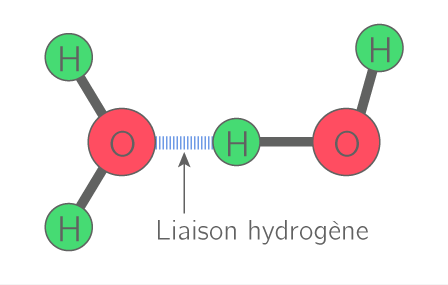
\includegraphics[scale = 0.5]{liaison_H.png}
	\end{center}
	\caption{Liaison hydrogène entre deux molécules d'eau.}
	\end{figure}

	\item La liaison est dirigée, l'angle étant égal à 180$\degree$.\\
	
	\item On retiendra l'ordre de grandeur de l'énergie associée à cette liaison : 10 à 40 kJ/mol, 			ce qui est plus important que les interactions de van der Waals, mais nettement plus faible que 		les énergies en jeu dans les liaisons covalentes.
\end{itemize}

\subsubsection{Conséquences}

\begin{itemize}
	\item \textbf{Structure de la glace :} la glace, quelle que soit sa structure 							cristallographique, est formée d'un assemblage régulier de molécules d'eau qui utilisent, 				chacune, leurs possibilités d'établir des liaisons hydrogène. Chaque atome d'oxygène, pris 				individuellement, se trouve localisé au centre d'un tétraèdre dont les sommets sont occupés par 		les atomes d'oxygène de quatre autres molécules d'eau. Il en résulte une structure rigide et 			lacunaire, occupant plus de volume qu'à l'état liquide : la glace est par conséquent moins dense 	que l'eau liquide. Lorsqu'on réchauffe de la glace, elle fond à 0$\degree$ C sous pression 				atmosphérique. La masse volumique de l'eau liquide augmente de 0$\degree$ C jusqu'à 4$\degree$ 			C, résultant de l'effondrement progressif des liaisons hydrogène. Au delà de 4 degrés, la masse 		volumique diminue avec la température, comme pour la plupart des autres corps purs.\\
	
	\begin{figure}[h!]
	\begin{center}
	\begin{tabular}{cc}
	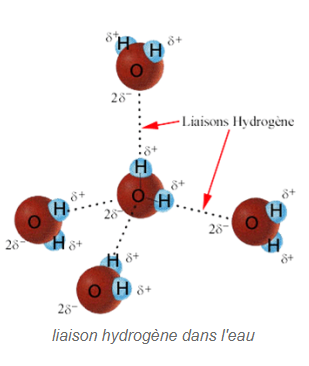
\includegraphics[scale = 0.7]{glace_H.png}
	&
	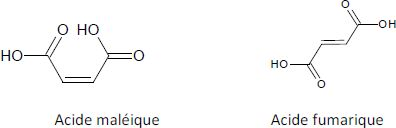
\includegraphics[scale = 0.8]{fumaleic.png}
	\end{tabular}
	\end{center}
	\caption{Gauche : arrangement des molécules d'eau dans la glace ; droite : acides maléique et 			fumarique.}
	\end{figure}	
	
	\item \textbf{Températures de fusion et d'ébullition :} la liaison hydrogène, de nature 				attractive, est stabilisatrice et lorsque les molécules d'un corps pur peuvent établir entre 			elles de telles liaisons, cela élève leurs \textbf{températures de fusion et d'ébullition}. On 			explique ainsi les valeurs élevées observées pour l'eau, l'ammoniac et le fluorure d'hydrogène 			dans le second tableau de la figure 4.\\
	
	Certaines molécules, comme l'\textbf{acide maléique}, peuvent former des liaisons hydrogène 			intramoléculaires, "consommant" la possibilité d'établir ces liaisons avec leurs voisines. Ceci 		explique pourquoi l'acide maléique et l'acide fumarique, stéréoisomères (même formule brute, 			arrangement des atomes différent), ont des températures de changement d'état différentes, celles 	de l'acide fumarique étant les plus élevées. Chaque molécule d'acide fumarique peut participer à 	davantage de liaisons hydrogène intermoléculaires que l'acide maléique.\\
	
	\item \textbf{Résistance de certains matériaux} : bien que la liaison hydrogène soit une liaison 	faible, un grand nombre de ces liaisons suffit à donner des propriétés de résistance mécanique 			remarquables à certains composés. On citera le Kevlar, polymère organique utilisé entre autres 			pour les gilets pare-balles. Ce polymère est constitué de chaînes parallèles, reliées entre 			elles par liaison hydrogène.
\end{itemize}

\newpage
\section{Les solvants}\label{sec:2}

\subsection{Définition}

Un solvant est un \textbf{fluide} (liquide ou supercritique) permettant d'\textbf{obtenir une solution} par \textbf{dissolution} d'un composé chimique, qu'on appelle \textbf{soluté}. D'une solution, c'est l'espèce majoritaire (et de loin).

\subsection{Propriétés et classification}

Nous allons maintenant discuter des caractéristiques physiques des solvants, à la lumière de ce que nous avons vu au sujet des liaisons faibles.

\subsubsection{Pouvoir dispersant}

La permittivité diélectrique relative du solvant intervient dans l'énergie d'interaction entre deux ions de charge $Z_1e$ et $Z_2e$ situés à une distance $r$
\begin{equation}
	U(r) = \frac{Z_1 Z_2 e^2}{4\pi\epsilon_0 \epsilon_r r}.
\end{equation}
Cette interaction est d'autant plus faible qu'$\epsilon_r$ est élevée : un solvant de forte permittivité diélectrique ($\epsilon_r > 40$) est dit \textbf{dispersant}. Les ions sont alors bien dispersés et interagissent peu entre eux. Dans un solvant de faible permittivité ($\epsilon_r < 20$), donc \textbf{non dissociant}, les ions restent associés sous forme de paires d'ions (ou d'agrégats d'ions).

\subsubsection{Polarité}

Un solvant possédant un fort moment dipolaire est capable de favoriser la dissolution des composés ioniques, comme le chlorure de sodium. Il stabilisera bien les ions, via des interactions ion-dipôle, ainsi que les molécules polaires, via des interactions dipôle-dipôle.

\begin{figure}[h!]
	\begin{center}
	\begin{tabular}{|c|c|c|}
		\hline
		Composé & $\mu (D)$ & $\epsilon_r$ \\
		\hline
		Cyclohexane & 0 & 2.0\\
		\hline
		Éther diéthylique & 1.15 & 4.2\\
		\hline
		Acétone & 2.88 & 20.7\\
		\hline
		Éthanol & 1.69 & 24.8\\
		\hline 
		Eau & 1.85 & 78.5\\
		\hline
	\end{tabular}	
	\end{center}
	\caption{Classement par ordre de polarité croissante de plusieurs solvants : 
	\textcolor{blue}{alcanes $<$ éthers $<$ cétones $<$ alcools $<$ acides carboxyliques $<$ eau}.}
\end{figure}	

De façon générale, les solvants polaires ont une importante permittivité diélectrique et un fort moment dipolaire.

\subsubsection{Proticité}

Un solvant protique possède un ou plusieurs \textbf{atomes d'hydrogène susceptibles de s'associer par liaison hydrogène} avec le soluté. Un solvant ne possédant pas cette particularité est dit \textbf{aprotique}. On soulignera les \textbf{propriétés particulières de l'eau} : ce solvant est fortement dissociant, fortement polaire et de surcroît, protique.

\newpage
\subsection{Dissolution}

La dissolution d'un composé dans un solvant consiste à le disperser tout en créant à son voisinage une couche de solvatation : il s'entoure de molécules de solvant avec qui il interagit pour se stabiliser. \textbf{Plusieurs phénomènes peuvent intervenir alors}, si les propriétés du solvant le permettent. Dans le cas de la dissolution du chlorure d'hydrogène HCl dans l'eau, nous aurons :

\begin{itemize}
	\item \textbf{Ionisation :} création d'une paire d'ions
	\begin{equation}
		\text{HCl} = \text{H}^+ {}^-\text{Cl},
	\end{equation}
	\item \textbf{Dispersion :} séparation de la paire
	\begin{equation}
		\text{H}^+ {}^-\text{Cl} = \text{H}^+ \text{Cl}^-
	\end{equation}		
	\item \textbf{Solvatation :} : les ions et le solvant établissent des interactions attractives 			stabilisatrices (dipôle-ion dans le cas présent, mais Van der Waals et liaisons hydrogène avec 			d'autres solutés).
	\begin{equation}
		\text{H}^+ \text{Cl}^- = \text{H}^+ \text{Cl}^-
	\end{equation}	 
\end{itemize}

Le résultat obtenu est une solution d'acide chlorhydrique. Dans un solvant apolaire, seule la solvatation aura lieu. Dans un solvant peu dissociant, il n'y aura pas de dispersion. Il n'y aura pas d'ionisation pour un composé au caractère fortement ionique, comme le chlorure de sodium NaCl.\\

Un solvant dissout bien un soluté si solvant et soluté ont des propriétés de polarité et de proticité semblables, ainsi on va considérer \textbf{trois grandes catégories de solvants} :
\begin{itemize}
	\item les solvants \textbf{polaires protiques} : ils solvatent bien les anions (grâce aux 				liaison hydrogène) ainsi que les molécules polaires. On peut citer l'eau, l'éthanol, le 1,3-			propanediol (qui peut être produit à partir du maïs et qui est biodégradable);\\
	\item les solvants \textbf{polaires aprotiques} : ils solvatent bien les cations, ainsi que les 		molécules polaires, moins bien les anions. On peut citer la DMSO (diméthylsulfoxyde) et la 				propanone (acétone);\\
	\item les solvants \textbf{apolaires aprotiques} : ils sont non dispersants et solvatent donc 			mal les ions et les composés polaires. Ils solvatent bien les composés apolaires via les 				interactions de dispersion. C'est le cas du cyclohexane, du toluène, du THF (tétrahydrofurane) 			ou du benzène (désormais proscrit en raison du risque CMR). Le 2-méthyltétrahydrofurane, produit 	à partir du sucre de canne, peut se substituer au THF et au toluène, d'origine pétrochimique.\\
\end{itemize}

On peut maintenant établir une règle qualitative : \textbf{les semblables dissolvent bien les semblables}. Cette règle reflète le fait que les interactions intermoléculaires soluté/soluté sont remplacées par des interactions soluté/solvant. Si ces nouvelles interactions sont de même nature que les anciennes, il faut peu d'énergie pour réaliser la mise en solution et la dissolution est favorable.\\

Pour mettre cette règle en évidence, mettons en œuvre une expérience, \textcolor{red}{celle de la dissolution du chlorure de sodium dans différents solvants :}
\begin{figure}[h!]
	\begin{center}
	\begin{tabular}{|c|c|c|c|c|}
		\hline
		Solvant    & Cyclohexane & Éthanol & Acétone & Eau \\
		\hline
		Dispersant & Non & Non & Oui & Oui \\
		\hline
		Polaire    & Non & Oui & Oui & Oui \\
		\hline
		Protique   & Non & Oui & Non & Oui \\
		\hline
		Résultat   &  &  &  &  \\
		\hline 
	\end{tabular}	
	\end{center}
	\caption{Tableau des résultats de l'expérience.}
\end{figure}	

\subsection{Miscibilité}

De la même manière : deux solvants dont les molécules possèdent des \textbf{propriétés de polarité comparables seront, en général miscibles}. Un mélange des deux conduira à l'observation d'une seule phase liquide.\\

Deux solvants non-miscibles formeront des phases distinctes, séparées par une interface. C'est le cas de l'eau et du cyclohexane, par exemple.\\


\textcolor{red}{Extraction du diiode de la bétadine dans une ampoule à décanter :} le diiode est le principe actif de la bétadine, complexé par la povidone. Le diiode est une molécule apolaire, donc peu soluble dans l'eau, mais bien plus soluble dans le cyclohexane (lui aussi apolaire). On introduit quelques gouttes de bétadine dans de l'eau contenue dans une ampoule à décanter. L'eau prend une coloration orangée. On introduit ensuite un volume de cyclohexane, moins dense que l'eau. L'interface entre les deux solvants se forme, et rapidement le cyclohexane prend une teinte violette, signe que le diiode passe en phase organique. On agite l'ampoule à décanter, robinet ouvert vers le haut, puis on referme le robinet et on laisse décanter. Si on a introduit suffisamment peu de diiode, l'eau redevient incolore et la phase organique devient violette, traduisant la préférence du diiode pour un solvant apolaire.

\begin{figure}[h!]
\begin{center}
	\begin{tabular}{cc}
		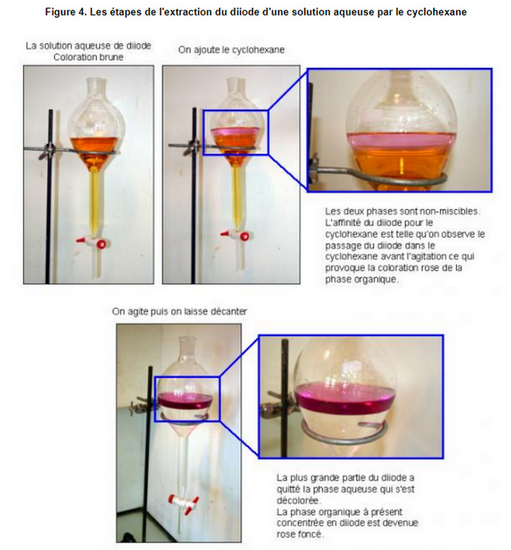
\includegraphics[scale = 0.95]{i2_cyclo.png}
	\end{tabular}
\end{center}
\caption{Extraction du diiode par le cyclohexane.}
\end{figure}	
	
La plus grande partie du diiode a migré de la phase aqueuse vers la phase organique. Si on rajoute de la bétadine dans l'ampoule, on remarque qu'il arrive un moment où la coloration orangée de la phase aqueuse persiste : \textbf{le soluté se répartit entre les deux phases}.	
	
\section{Extraction liquide-liquide et équilibre de partage}\label{sec:3}

L'opération d'extraction liquide-liquide est une technique largement utilisée en chimie.
Elle intervient en général à la fin d'une synthèse pour traiter un brut réactionnel liquide,
c'est à dire un mélange qui contient le produit de la réaction, les produits secondaires, les réactifs en excès et le solvant.\\

Le but est d'isoler le produit d'intérêt solvaté initialement dans un solvant S en le faisant passer dans une phase organique ou aqueuse (solvant S' : on fait passer la substance d'un solvant à un autre. L'extraction n'est possible que si les deux liquides ne sont pas miscibles. Bien entendu, le produit d'intérêt doit avoir la meilleure différence possible d'affinité entre les deux solvants.\\

Lorsqu'on introduit un soluté A dans un milieu contenant deux phases liquides non miscibles en contact, il s'établit un \textbf{équilibre de partage} : 
\begin{equation}
	\boxed{A(S) \rightleftarrows A(S')}.
\end{equation}
\textbf{Le soluté se répartit dans les deux phases}, \textbf{en proportions compatibles avec le coefficient de partage}
\begin{equation}
	{K\degree}(T) \equiv \frac{a(A(S'))}{a(A(S))} = \frac{[A]_{S'}}{[A]_S}
\end{equation}
constante thermodynamique de l'équilibre de partage, fonction de la température T.

\subsection{Extraction de l'acide benzoïque par l'huile de tournesol}
Possibilité 1 : chimie verte.

Nous nous proposons de réaliser la détermination d'une constante de partage, celle de l'acide benzoïque se partageant entre une phase aqueuse et une (huile de tournesol) :
\begin{equation}
	\boxed{K\degree (T) = \frac{[\text{PhCOOH}]_\text{orga}}{[\text{PhCOOH}]_\text{huile}}.}
\end{equation}

\begin{figure}[h!]
\begin{center}
	\begin{tabular}{cc}
		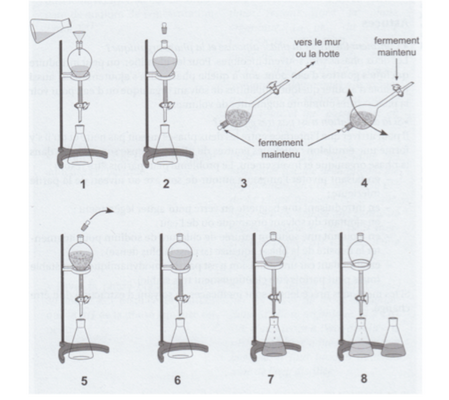
\includegraphics[scale = 0.85]{ampoule.png}
	\end{tabular}
\end{center}
\caption{Protocole pour l'extraction liquide-liquide suivie de la décantation.}
\end{figure}

\begin{itemize}
	\item \textbf{Matériel :}
	\begin{itemize}
		\item Acide benzoïque (s $=$ 2.9 g/L à 25$\degree$ C dans l'eau, M $=$ 122.1 g/mol,
		 pKa $=$ 4.2) : préparer 200 mL de solution saturée $S_0$.
		\item Extraction d'un volume de $V_0 =$ 50 mL de la solution $S_0$ par 25 mL d'huile de 				colza avec ampoule à décanter. Identification des deux phases (densité, couleur). 						Séparation des deux phases.
		\item Dosage colorimétrique de la phase aqueuse en utilisant le BBT. Calcul des 						concentrations dans les deux phases et obtention de $K\degree$.\\
	\end{itemize}
	
	\item \textbf{Exploitation :}
	\begin{itemize}
		\item Calcul de la concentration en phase aqueuse :
		
		\item Calcul de la concentration en phase organique :
		
		\item Calcul de la constante de partage
	\end{itemize}
\end{itemize}

\subsection{Extraction de l'acide propanoïque par l'éther diéthylique}
Voir Chavanne, p152

\begin{itemize}
	\item \textbf{Matériel}
	\begin{itemize}
		\item Ampoule à décanter de 125 mL;
		\item Solution d'acide propanoïque à 1 mol/L (M = 74.08 g/mol ; pKa $=$ 4.87 à 25\degree C ; 						18.5g dans 250 mL d'eau);
		\item Solution d'hydroxyde de sodium à 0.5 mol/L \textbf{titrée};
		\item Phénophtaléine
		\item Burette graduée (25 ou 30 mL), agitateur magnétique
	\end{itemize}
	
	\item \textbf{Préparation : dosage de $\mathcal{S}_0$}
		Prélever 10 mL de solution $\mathcal{S}_0$, doser par la soude en présence de phénolphtaléine. 				Indication :
		\begin{equation}
			V_\text{eq} = 20 mL.
		\end{equation}
		
	\item \textbf{Préparation : extraction liquide-liquide}
	\begin{itemize}
		\item Introduire $V_\text{eau} =$ 25 mL de solution d'acide propanoïque, puis $V_\text{org} =$ 			45 mL d'éther diéthylique. Agiter vigoureusement 5 minutes, en dégazant de temps en temps 				(évacuation de la surpression générée par l'agitation).
		\item Laisser reposer.\\
	\end{itemize}
	
	\item \textbf{Préparation : séparation}
	\begin{itemize}
		\item Séparer la phase aqueuse de la phase organique (qui surnage, éther moins dense).\\
	\end{itemize}
	
	\item \textbf{Direct : dosage de la phase aqueuse}
	\begin{itemize}
		\item Prélever 10, 15 voire 20 mL de phase aqueuse.
		\item Doser par la soude, en présence de phénolphtaléine.
		\item Indication : $V_\text{eq} =$ 3.52 mL pour 10 mL prélevés.\\
	\end{itemize}
	
	\item \textbf{Direct : exploitation}
	\begin{itemize}
		\item Remonter à la concentration $[\text{Acide}]_\text{(aq)}$ grâce au volume équivalent.
		\item Calculer la quantité de matière dans la phase organique :
			\begin{equation}
				C_0 V_\text{eau} = n(A)_\text{org} + [\text{Acide}]_\text{(aq)} V_\text{eau}. 
			\end{equation}
		\item Remonter à la concentration en phase organique $n(A)_\text{org}/V_\text{org}$ puis à la 					constante de partage \textcolor{blue}{(mesurer la température)} à la température 						ambiante.
		\item Calculer le rendement de l'extraction : concentration dans la phase organique sur 						concentration initiale en phase aqueuse.
	\end{itemize}
	
	\item \textbf{Remarques à faire}
	\begin{itemize}
		\item On néglige la dissociation de l'acide dans l'eau (c'est un acide faible);
		\item On néglige la miscibilité de l'éther avec l'eau, qui n'est pas si négligeable que ça.
	\end{itemize}
\end{itemize}

\newpage
\section*{Conclusion}

Une très grande majorité de solvants organiques sont des composés volatiles, pouvant se disperser dans l'atmosphère. Ils ont par ailleurs comme défaut d'être toxiques et inflammables. La chimie verte a notamment pour but de concevoir des produits et des procédés chimiques permettant de réduire voire d'éliminer l'utilisation et la synthèse de substances dangereuses.\\

L'eau est le solvant renouvelable et non toxique par excellence, mais nous avons vu qu'elle n'était pas capable de solvater correctement un grand nombre de substances organiques (souvent faiblement polaires voire totalement apolaires). Le développement de solvants non toxiques à partir de ressources renouvelables (et non issues de la pétrochimie comme c'est actuellement le cas) est l'un des objectifs de la chimie verte, de même que la réduction des quantités de solvant utilisées.\\

Le caractère "vert" d'un solvant dépend de plusieurs critères : sa toxicité, les risques que l'on encourt à le manipuler, sa réactivité, sa capacité à le recycler, son coût. Les recherches actuelles étudient plusieurs pistes :
\begin{itemize}
	\item les réactions sans solvants, en phase gazeuse avec catalyse solide,
	\item les fluides supercritiques (notamment le dioxyde de carbone).
\end{itemize}

\end{document}